
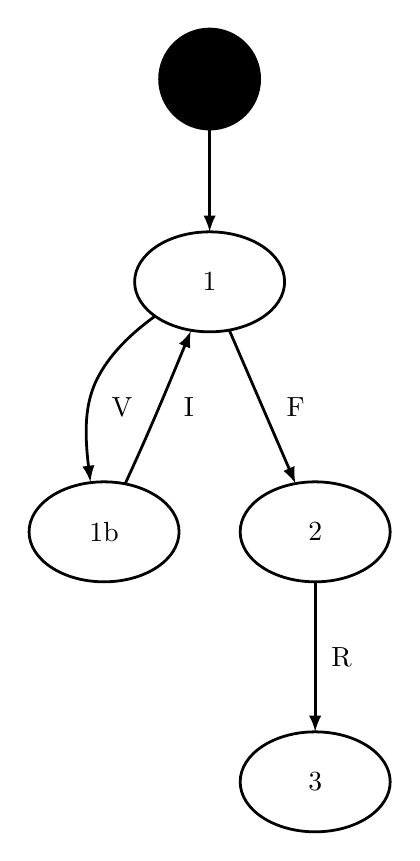
\begin{tikzpicture}[>=latex,line join=bevel,]
  \pgfsetlinewidth{1bp}
%%
\pgfsetcolor{black}
  % Edge: 1b -> 1
  \draw [->] (34.609bp,125.33bp) .. controls (37.305bp,131.2bp) and (40.33bp,137.88bp)  .. (43bp,144bp) .. controls (46.777bp,152.66bp) and (50.777bp,162.19bp)  .. (58.215bp,180.23bp);
  \definecolor{strokecol}{rgb}{0.0,0.0,0.0};
  \pgfsetstrokecolor{strokecol}
  \draw (57.5bp,153bp) node {I};
  % Edge: 0 -> 1
  \draw [->] (65bp,252.81bp) .. controls (65bp,244.79bp) and (65bp,235.05bp)  .. (65bp,216.03bp);
  % Edge: 1 -> 1b
  \draw [->] (45.274bp,185.58bp) .. controls (37.087bp,179.69bp) and (28.468bp,171.69bp)  .. (24bp,162bp) .. controls (20.323bp,154.03bp) and (19.798bp,144.65bp)  .. (22.082bp,126bp);
  \draw (33.5bp,153bp) node {V};
  % Edge: 1 -> 2
  \draw [->] (72.148bp,180.45bp) .. controls (77.667bp,167.66bp) and (85.41bp,149.74bp)  .. (95.885bp,125.48bp);
  \draw (96bp,153bp) node {F};
  % Edge: 2 -> 3
  \draw [->] (103bp,89.614bp) .. controls (103bp,77.24bp) and (103bp,60.369bp)  .. (103bp,36.05bp);
  \draw (112.5bp,63bp) node {R};
  % Node: 1
\begin{scope}
  \definecolor{strokecol}{rgb}{0.0,0.0,0.0};
  \pgfsetstrokecolor{strokecol}
  \draw (65bp,198bp) ellipse (27bp and 18bp);
  \draw (65bp,198bp) node {1};
\end{scope}
  % Node: 0
\begin{scope}
  \definecolor{strokecol}{rgb}{0.0,0.0,0.0};
  \pgfsetstrokecolor{strokecol}
  \definecolor{fillcol}{rgb}{0.0,0.0,0.0};
  \pgfsetfillcolor{fillcol}
  \filldraw [opacity=1] (65bp,271bp) ellipse (18bp and 18bp);
\end{scope}
  % Node: 2
\begin{scope}
  \definecolor{strokecol}{rgb}{0.0,0.0,0.0};
  \pgfsetstrokecolor{strokecol}
  \draw (103bp,108bp) ellipse (27bp and 18bp);
  \draw (103bp,108bp) node {2};
\end{scope}
  % Node: 1b
\begin{scope}
  \definecolor{strokecol}{rgb}{0.0,0.0,0.0};
  \pgfsetstrokecolor{strokecol}
  \draw (27bp,108bp) ellipse (27bp and 18bp);
  \draw (27bp,108bp) node {1b};
\end{scope}
  % Node: 3
\begin{scope}
  \definecolor{strokecol}{rgb}{0.0,0.0,0.0};
  \pgfsetstrokecolor{strokecol}
  \draw (103bp,18bp) ellipse (27bp and 18bp);
  \draw (103bp,18bp) node {3};
\end{scope}
%
\end{tikzpicture}

